
\section{Elemente de configurare}

Pentru compilarea și link-editarea aplicației a fost folosit Visual Studio 2022. Standardul C++ folosit este ISO C++ 17. Trebuie folosite anumite definiții preprocesor pentru compilarea aplicației. Mai jos sunt enunmerate definițiile preprocesor folosite și motivul pentru care acestea au fost folosite:

\begin{itemize}
\item HAVE\_ZLIB: Încărcarea datelor volumetrice de tip NIfTI arhivate (.nii.gz);
\item USE\_BOOKMARK: Compilarea cu success a bibliotecii externe ImGuiFileDialog. Această opțiune permite salvarea locațiilor favorite în memorie pentru încărcarea ușoară a datelor volumetrice;
\item \_SILENCE\_ALL\_CXX17\_DEPRECATION\_WARNINGS: Sunt folosite funcții depreciate în standardul C++ 17 în biblioteci folosite;
\item \_CRT\_NONSTDC\_NO\_DEPRECATE: Compilarea bibliotecii gzlib. Funcțiile open, read, write și close sunt marcate ca fiind depreciate;
\item \_CRT\_SECURE\_NO\_DEPRECATE: Biblioteca ImGuiFileDialog folosește funcții nesigure precum sscanf.
\end{itemize}.

Trebuie incluse următoarele biblioteci în directorul "extern": niftilib, zlib, znzlib, freeglut, ImGui, ImGuiFileDialog și libtorch (versiunea pentru CPU). De asemenea sunt necesare dll-ul și lib-ul pentru freeglut amplasate în directorul principal cu fișierul proiect.

Utilizarea interfeței utilizator este prezentată în capitolul anterior. Parametrii transformărilor de rotație, translație și tăiere pot fi manipulați folosind și mouse-ul și tastatura. Cu mișcări ale mouse-ului pe axa Ox va fi rotit volumul pe axa Ox, similar pentru axa Oy. Prin mișcarea rotiței mouse-ului se modifică scara la care este vizualizat volumul. Rotația poate fi efectuată și cu apăsarea tastelor 'w', 'a', 's' și 'd' sau a săgeților de pe tastatură. Pentru aplicarea translației vor fi folosite aceleași taste ca pentru rotație atunci când este apăsată concomitent tasta ALT.


\section{Rezultate obținute în aplicația de redare}

\begin{figure}[!h]
    \centering
    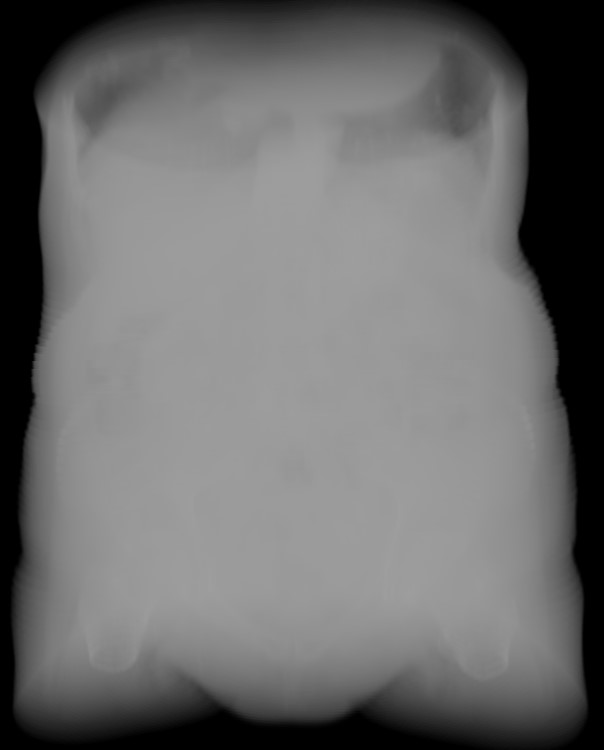
\includegraphics[width=7cm]{images/vol_wo_tf.jpg}
    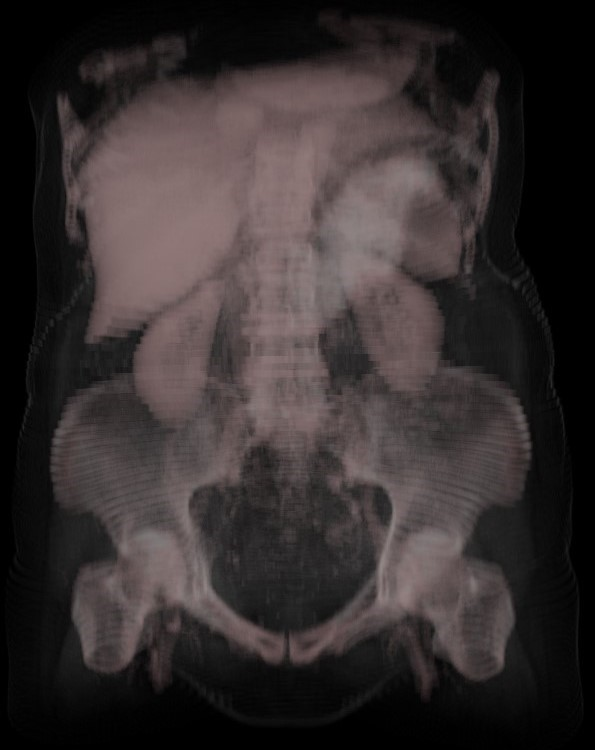
\includegraphics[width=7cm]{images/vol_w_tf.jpg}
    \\
    \caption{Comparație intre redarea unui volum fară a fi folosită o funcție de transfer (stangă) și cu o funcție de transfer (dreapta).}
    \label{fig:comp_tf}
\end{figure}

În figura \ref{fig:comp_tf} se poate observa importanța funcției de transfer în vizualizarea volumelor. Pentru a putea reda o imagine semnificativă utilizatorului trebuie furnizată sau creată o funcție de transfer care să filtreze detaliile nesemnificative și să faciliteze vizualizarea regiunilor de interes. În figura \ref{fig:comp_tf} a fost folosită o funcție simplă, dar pentru a obține rezultate mai bune ar putea fi explorate metode de ghidare a utilizatorului în căutarea unei funcții de transfer  optime\cite{Zhou2009AutomaticTF}.

\begin{figure}[!htb]
    \centering
    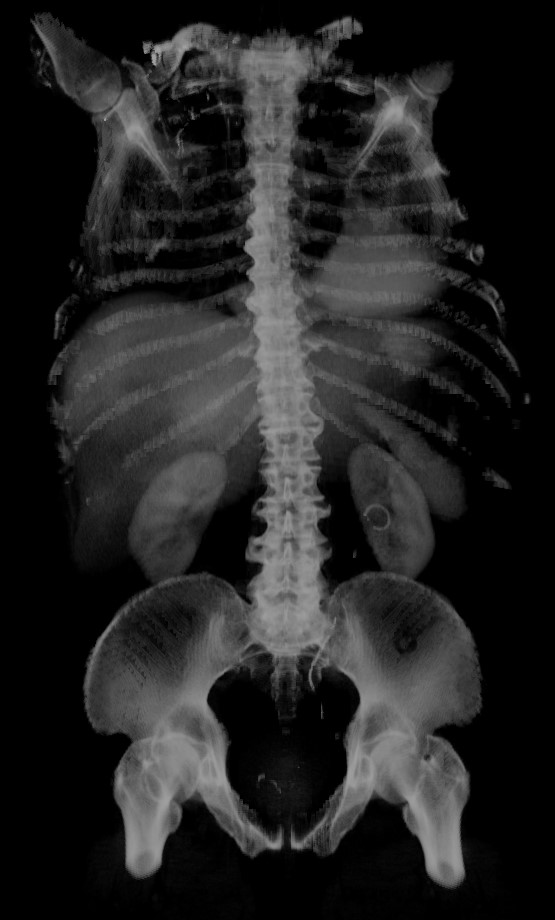
\includegraphics[width=5cm]{images/seg_comp.jpg}
    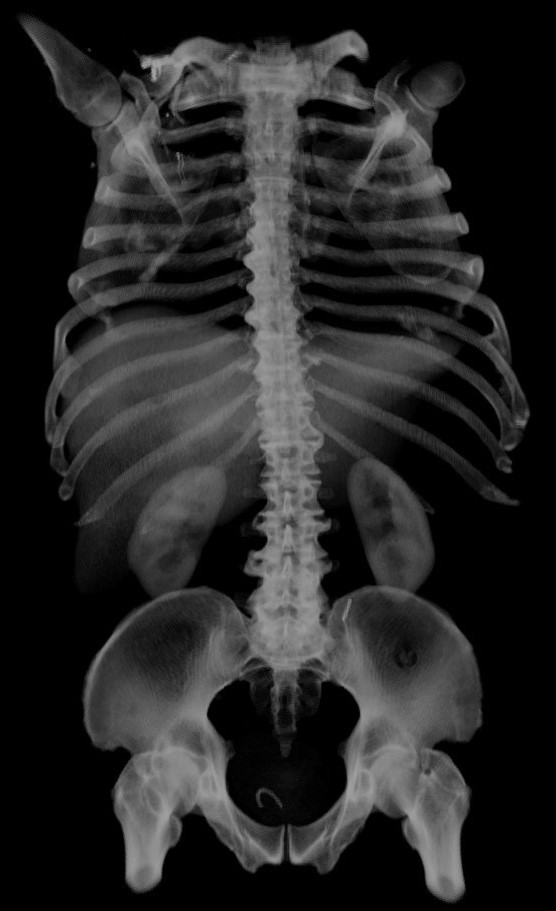
\includegraphics[width=5cm]{images/seg_labels.jpg}
    \\
    \caption{Comparație dintre segmentarea obținută cu ajutorul modelului de segmentare (stânga) și cea manuală din setul de date (dreapta) pentru aceeași imagine volumetrică. Redarea a fost realizată utilizând aplicația de redare fară aplicarea unei funcții de transfer și folosind aceeași parametri de vizualizare.}
    \label{fig:viz_seg_comp}
\end{figure}

În figura \ref{fig:viz_seg_comp} este prezentat în partea stangă rezultatul aplicării unei măști de segmentare generate automat de către aplicație. Pentru obținerea unei astfel de măști sunt necesare resurse suplimentare precum mult mai multă memorie RAM (aproximativ de patru ori mai multă memorie decât este necesar doar pentru vizualizare) și timp de procesare extins (în funcție de dimensiunea volumului de date poate dura și câteva minute pentru obținerea măștii de segmentare).


\section{Rezultate experimentale obținute în antrenarea modelului de segmentare semantică}

Pot fi folosite anumite metrici pentru a studia eficacitatea unui model. Pentru clasificare poate fi calculată acuratețea, adică procentajul punctelor etichetate corect. Dar, această măsură nu este potrivită în contextul segmentării imaginilor volumetrice, deoarece o mare parte dintre punctele din volum nu sunt etichetate. O soluție ar fi folosirea măsurii F care este calculată astfel:
\begin{equation}
    F_1 = \frac{tp}{tp + \frac{1}{2}(fp + fn)},
\end{equation}
unde
\begin{itemize}
  \item[] tp \textit{true positives} reprezintă numărul de puncte etichetate corect.
  \item[] fp \textit{false positives} reprezintă numărul de puncte etichetate în mod eronat.
  \item[] fn \textit{false negatives} reprezintă numărul de puncte neetichetate în mod eronat.
\end{itemize}


\begin{figure}[!htb]
    \centering
    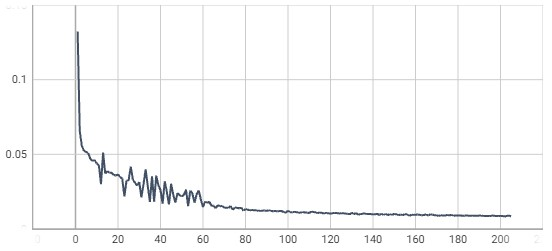
\includegraphics[width=8cm]{images/seg_train_results/training_loss.jpg}
    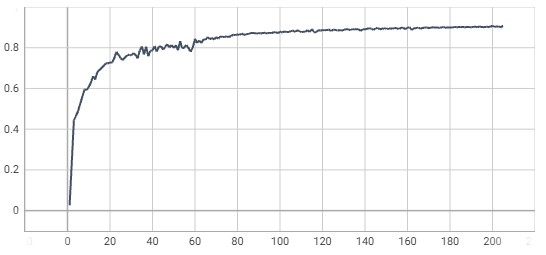
\includegraphics[width=8cm]{images/seg_train_results/training_f1.jpg}
    \\
    \caption{Valorile funcției cost și a măsurii F1 calculate pentru setul de date de antrenare pe parcursul antrenării.}
    \label{fig:res_training}
\end{figure}

\begin{figure}[!htb]
    \centering
    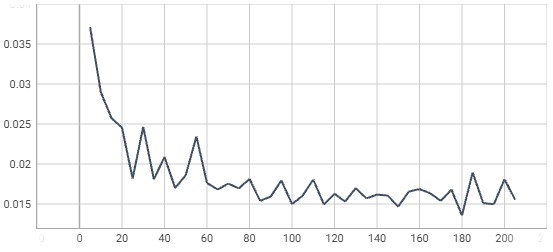
\includegraphics[width=8cm]{images/seg_train_results/validation_loss.jpg}
    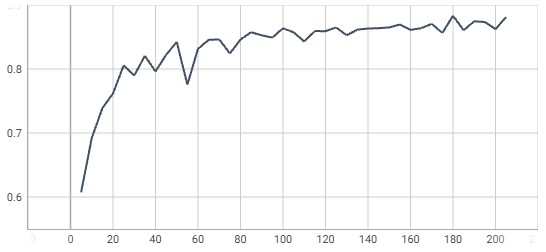
\includegraphics[width=8cm]{images/seg_train_results/validation_f1.jpg}
    \\
    \caption{Valorile funcției cost și a măsurii F1 calculate pentru setul de date de validare pe parcursul antrenării.}
    \label{fig:res_validation}
\end{figure}

\begin{figure}[!htb]
    \centering
    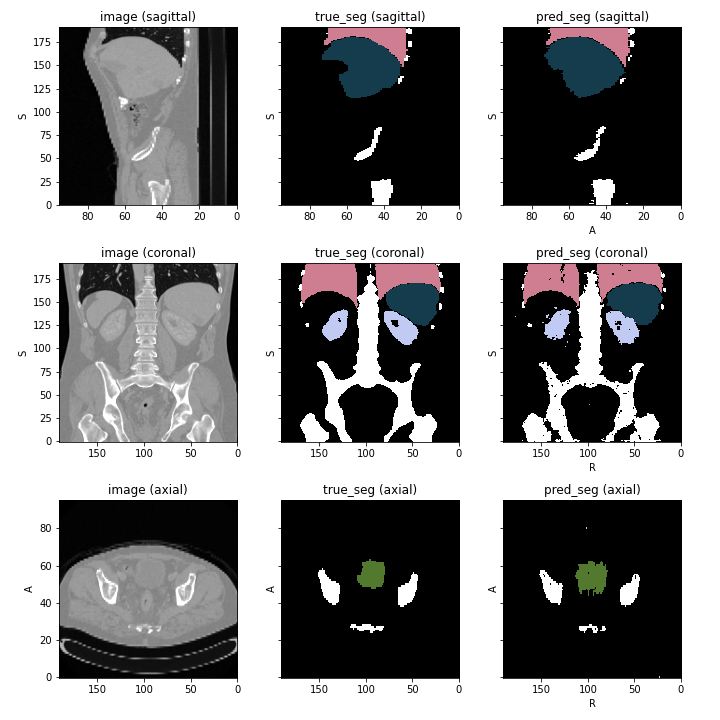
\includegraphics[width=15cm]{images/seg_train_results/041.png}
    \\
    \caption{O porțiune dintr-o imagine volumetrică din setul de date de validare. În stânga este reprezentată imaginea propriu zisă, în mijloc este segmentarea manuală din setul de date și în dreapta este segmentarea automată.}
    \label{fig:results_pytorch}
\end{figure}

La finalul antrenării, au fost folosite 21 de imagini din setul de date pentru a calcula eficacitatea modelului pe un set de date de test. Valoarea funcției F1 rezultată în etapa de testare este 0.89, puțin mai mare decât 0.88 obținută pentru setul de date de validare și puțin mai mică decât 0.90 obținută pentru setul de date folosit la antrenare. Luând în considerare aceste valori poate fi observată o capacitate de generalizare a modelului pentru date neîntâlnite în antrenarea sa. Acest fapt este de dorit pentru folosirea cu succes în practică a modelului. În figurile \ref{fig:res_training} și \ref{fig:res_validation} sunt prezentate rezultatele antrenării modelului final, obținut în urma experimentării cu mai multe arhitecturi și diferiți parametri. Modelul folosit în final este cel implementat în biblioteca MONAI care a fost antrenat fară a fi folosite petice disjuncte din imaginile din setul de date. Cu această metodă a fost obținut un model care poate generaliza mai bine într-un timp mai scurt de antrenare decât alternativele explorate pe parcursul experimentării. În figurile \ref{fig:results_pytorch} și \ref{fig:viz_seg_comp} sunt reprezentări vizuale ale rezultatului antrenării, putând fi observată similitudinea dintre masca de segmentare realizată manual și cea generată de către rețeaua neuronală. În figura \ref{fig:results_pytorch} sunt afișate felii din volum și măștile de segmentare în aceleași poziții, iar în figura \ref{fig:viz_seg_comp} sunt redări obținute cu ajutorul aplicației de vizualizare realizată în cadrul proiectului.

\begin{figure}[!htb]
    \centering
    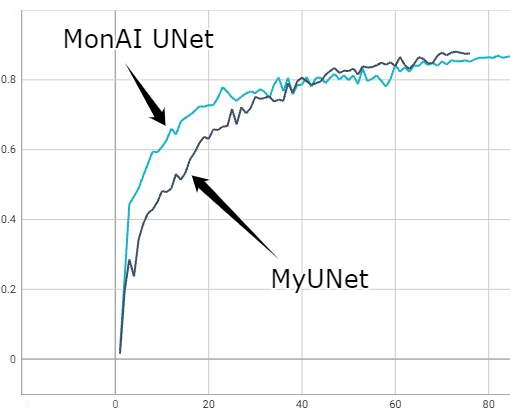
\includegraphics[width=8cm]{images/seg_train_results/UNET_train_comp.png}
    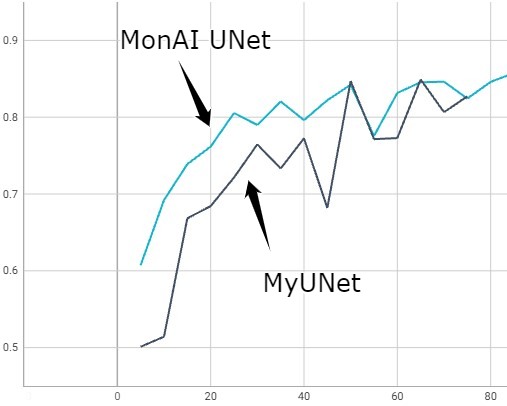
\includegraphics[width=8cm]{images/seg_train_results/UNET_valid_comp.png}
    \\
    \caption{Comparație a valorilor funcției F1 între implementarea UNet din biblioteca MONAI și implementarea din anexa \ref{appendix:30_model_unet3d_py} pe parcursul antrenării (stangă) și validării (dreapta).}
    \label{fig:comp_unet}
\end{figure}

\begin{figure}[!htb]
    \centering
    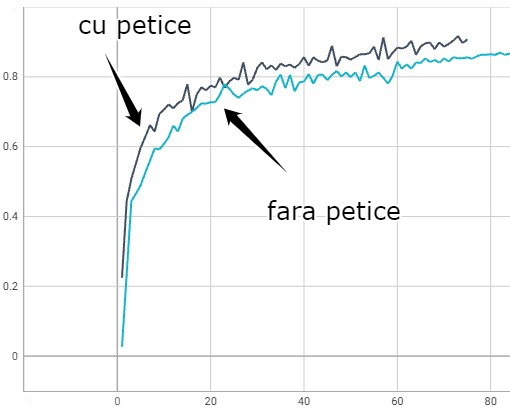
\includegraphics[width=8cm]{images/seg_train_results/patches_train_comp.png}
    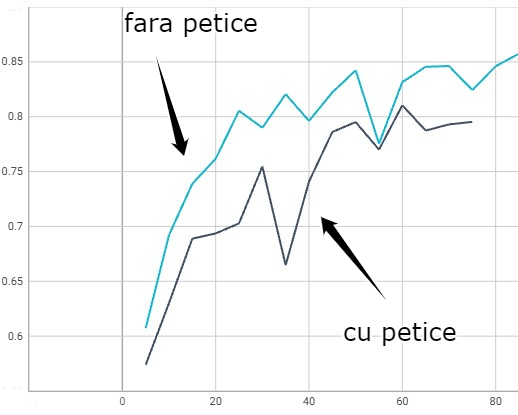
\includegraphics[width=8cm]{images/seg_train_results/patches_valid_comp.png}
    \\
    \caption{Comparație a valorilor funcției F1 intre metoda partitionarii intrării pe baza de petice și cea în care toată imaginea este primită la intrare de către rețeaua neurală. În stânga sunt valori pe parcursul antrenării, și în dreapta pentru etapa de validare.}
    \label{fig:comp_patches}
\end{figure}

În figura \ref{fig:comp_unet} este realizată o comparație între rezultatele antrenării a două arhitecturi de rețele neuronale similare folosind parametrii de antrenare asemănători. Trebuie menționat faptul că o epocă de antrenare pentru rețeaua din biblioteca MONAI este realizată mai rapid decât una pentru rețeaua din anexa \ref{appendix:30_model_unet3d_py}. Diferența principală dintre cele două implementări este că în MONAI UNet este implementat folosind principii de programare orientată obiect, pe când în cealaltă rețea sunt folosite liste de module din PyTorch pentru înlănțuirea blocurilor convolutionale. În figura \ref{fig:comp_patches} este realizată o comparație între o metodă de preprocesare a datelor și lipsa ei. Această metodă este împărțirea imaginilor din setul de date în petice disjuncte în scopul de a avea la intrarea rețelei imagini mai mici, astfel realizandu-se inferența și retropropagarea mai rapid. Un dezavantaj al acestei metode, după cum se poate observa și în figură este că sunt obținute rezultate mai slabe pe setul de validare, fapt ce arată că modelul antrenat pe petice de date nu generalizează la fel de bine.

